%! TEX root = kebutuhanmanusia.tex
% the main TeX file which is intended to compile, :VimtexReload after adjustment
   % this file should be included in the main file
% :h vimtex-tex-root
\documentclass[../manperil.tex]{subfiles}
%ensure the class of docs

\begin{document}

\section{Kebutuhan Manusia}%
\label{sec:Kebutuhan Manusia}
\subsection{Kebutuhan Manusia berdasarkan Abraham Maslow}%
\label{sub:Kebutuhan Manusia berdasarkan Abraham Maslow}


Berdasarkan teori ``Maslow’s Hirarchy of Needs" oleh Abraham Maslow terkait hirarkikebutuhan manusia digambarkan melalu piramida yang menyebutkan dari kebutuhanmanusia yang paling dasar atau rendah hingga mengerucut semakin ke atas. Hal ini dapatdiartikan tujuan kebutuhan manusia yang semakin lebih tinggi. Teori Abraham Maslow inimengedepankan sifat sosial yang ditinjau melalui psikologi humanistik. Penjelasan teoripiramida yang menggambarkan hirarki kebutuhan manusia tertuang dalam International Journal of Development and Economic Sustainability diantaranya sebagai berikut:


\begin{figure}
	\begin{center}
		
\includegraphics[width=.82\textwidth]{maslow_heirarchy}
		% filename may not contain space but _
	\end{center}
	\caption{Hirarki maslow }
	\label{fig:maslow}
\end{figure}


\subsubsection{Kebutuhan Psikologi}%
\label{ssub:Kebutuhan Psikologi}

Kebutuhan ini merupakan tingkatan yang paling dasar dari kebutuhan manusia ,kebutuhan fisiologi menjadi yang paling bawah karena kebutuhan ini merupakan aspekterpenting yang harus dipenuhi dalam kehidupan manusia seperti sandang, pangan danpapan. Oleh karenanya, pemenuhan yang layak berhak didapatkan oleh setiap individumanusia sebagai hal yang mendasar.

Penerapannya dalam bidang arsitektur adalah semua individu berhak mendapatnaungan atau ruang ( kebutuhan papan ) yang mampu mewadahi kebutuhan aktivitaspengguna didalamnya.
\begin{figure}
	\begin{center}
		
\includegraphics[width=.82\textwidth]{floating_schools_in_bangladesh}
		% filename may not contain space but _
	\end{center}
	\caption{Floating schools in bangladesh}
	\label{fig:school}
\end{figure}


\begin{itemize}
	\item Dalam arsitektur, tingkatan ini berkaitan dengan elemen-elemen mendasar yang diperlukan bagi kelangsungan hidup manusia.
	\item Ruang yang dirancang dengan baik akan memastikan akses ke cahaya alami, udara segar, air bersih, dan pengatur suhu.
	\item Tempat berlindung adalah kebutuhan dasar manusia, yang menekankan pentingnya menciptakan struktur untuk memberikan keselamatan, keamanan, serta perlindungan dari kondisi alam sekitar.
	\item Menyadari pentingnya pendidikan terlepas dari tantangan lingkungan, struktur terapung ini memastikan akses ke pendidikan tetap berjalan selama banjir.
	\item Dibangun di atas platform yang mengapung, sekolah-sekolah ini menyediakan ruang belajar yang aman dan kering, guna memenuhi kebutuhan fisiologis akan tempat berlindung dan keselamatan.
	\item Desain ini tidak hanya berfungsi sebagai respons yang tangguh terhadap tantangan langsung dari lingkungan, tetapi juga menekankan peran penting arsitektur dalam memastikan terpenuhinya kebutuhan dasar, bahkan dalam kondisi ekstrem.
\end{itemize}


\subsubsection{Safety Needs ( Kebutuhan Keamanan )}%
\label{ssub:safety_needs_(_kebutuhan_keamanan_)}

Kebutuhan ini merupakan tingkatan kedua yang menekankan kepada kebutuhan akanrasa aman dan keselamatan pada setiap individu manusia sehingga mampu memberikanrasa nyaman dan tentram pada aktivitas kehidupannya. Pada tingkatan ini dibidang arsitektur ialah bangunan tidak hanya sebagai tempatuntuk mewadahi atau memenuhi kebutuhan aktivitas manusia namun juga memberikan perlindungan didalamnya dari berbagai aspek sehingga manusia sebagai penggunadidalamnya memiliki rasa nyaman dan aman.A

\begin{figure}
	\begin{center}
		
\includegraphics[width=.82\textwidth]{cctv_tower_in_beijing}
		% filename may not contain space but _
	\end{center}
	\caption{CCTV Tower in Beijing}
	\label{fig:}
\end{figure}


\begin{itemize}
	\item Dalam istilah arsitektur, hal ini diterjemahkan menjadi menciptakan ruang yang mendukung keselamatan fisik, perlindungan dari bahaya lingkungan, dan rasa stabilitas.
	\item Bangunan harus kokoh secara struktural, dilengkapi dengan pintu keluar darurat, dan menyertakan fitur-fitur keamanan.
	\item Perencanaan wilayah dan kota memainkan peran penting dalam menyediakan lingkungan dan infrastruktur yang aman, memastikan bahwa penghuninya dapat beraktivitas di lingkungan mereka tanpa rasa takut.
	\item Dinding perimeter bangunan yang melingkar tanpa putus tidak hanya memberikan keselamatan fisik tetapi juga secara simbolis mewakili keamanan.
	\item Desain ini menciptakan lingkungan yang aman, baik secara fisik maupun psikologis, memenuhi kebutuhan keselamatan para penghuninya sekaligus memberikan pernyataan arsitektur yang berani.
\end{itemize}


\subsubsection{Kebutuhan Percaya dan Cinta Kasih}%
\label{ssub:cintah_kasih}

Kebutuhan ini menjelaskan mengenai manusia sebagai individu memiliki kebutuhanuntuk mencintai dan dicintai sehingga tercipta kepercayaan dan kedamaian di dalamhidupnya. Kebutuhan ini mencakup hal yang luas seperti perasaan seseorang untukmenjaga, peduli dan perhatian terhadap sesama maupun lingkungan disekitarnya yangdidasari atas rasa memiliki. Dalam arsitektur dapat diwujudkan dalam ruang yang mampu memfasilitasi danmewadahi kegiatan yang dapat menimbulkan rasa afeksi dan keakraban antar pengguna didalamnya sehingga terjalin sebuah perasaan yang timbul pada tiap individudidalamnya,hal ini dapat berupa perencanaan ruang komunal atau ruang publik yangdapat merefleksikan keakraban antar manusia.


\begin{figure}
	\begin{center}
		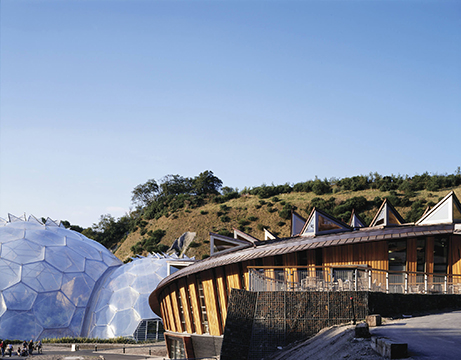
\includegraphics[width=.82\textwidth]{../figures/the_eden_project_in_cornwall.png}
		% filename may not contain space but _
	\end{center}
	\caption{The Eden Project in Cornwall, UK - Sir Nicholas Grimshaw
	}
	\label{fig:}
\end{figure}





\begin{itemize}
	\item Desain arsitektur dapat menumbuhkan hubungan sosial dengan menciptakan ruang komunal, seperti taman, plaza, dan pusat komunitas.
	\item Kompleks perumahan dapat dirancang untuk mendorong interaksi, dan kawasan multifungsi dapat menciptakan lingkungan yang hidup tempat orang-orang tinggal, bekerja, dan bersosialisasi di kawasan yang sama.
	\item Proyek ini mengubah bekas tambang tanah liat yang sudah tidak digunakan menjadi serangkaian bioma yang saling terhubung, menciptakan pusat pendidikan, kesadaran lingkungan, dan kegiatan komunal.
	\item Desain tersebut mendorong pengunjung untuk menjelajah dan berinteraksi, menumbuhkan rasa memiliki terhadap komunitas yang lebih besar yang menghargai keberlanjutan dan kesadaran lingkungan.
\end{itemize}

\subsubsection{Esteem Needs ( Kebutuhan untuk Dihargai )}%
\label{ssub:esteem_needs_(_kebutuhan_untuk_dihargai)}

Kebutuhan ini mengacu kepada capaian individu yang mengarah pada jenjangpekerjaan tertentu. Hasil perolehan dari capaian tersebut melahirkan kebutuhan individuuntuk menunjukkan derajatnya sehingga dapat dihargai dan dipercaya akan harga dirinyatersebut. Ada 2 jenis kebutuhan akan penghargaan diri , yang pertama berasal dari dirisendiri dan yang kedua berasal dari luar atau pengakuan lingkungan yang dapat berupaapresiasi,ketenaran dan lain sebagainya. Dalam arsitektur hal tersebut dapat digambarkan berupa kebutuhan orang akansebuah ruang atau bangunan yang mampu memberikan prestige pada penggunanyasehingga mampu memiliki sebuah penilaian yang baik akan harga dirinya.

\begin{figure}
	\begin{center}
		
\includegraphics[width=.82\textwidth]{the_burj_khalifa_in_dubai}
		% filename may not contain space but _
	\end{center}
	\caption{The Burj Khalifa in Dubai - Adrian Smith, SOM}
	\label{fig:}
\end{figure}


\begin{itemize}
	\item Dalam arsitektur, tingkatan ini dapat dipenuhi dengan menciptakan ruang yang mencerminkan identitas individu dan budaya.
	\item Ekspresi arsitektur melalui desain inovatif, motif budaya, serta perpaduan antara bentuk dan fungsi berkontribusi pada rasa bangga dan pencapaian.
	\item Bangunan ikonik dan tengara sering kali berfungsi sebagai simbol yang menanamkan rasa harga diri kolektif dalam suatu komunitas.
	\item Sebagai bangunan tertinggi di dunia, Burj Khalifa berdiri sebagai simbol pencapaian manusia dan kehebatan arsitektur.
	\item Desainnya berkontribusi pada harga diri kota Dubai dan para penduduknya, berfungsi sebagai tengara ikonik yang memperindah lanskap kota serta memperkuat rasa bangga dan pencapaian.
\end{itemize}

\subsubsection{Self Actualization ( Kebutuhan Akutualisasi Diri )}%
\label{ssub:self_actualization_(_kebutuhan_akutualisasi_diri_)}

Kebutuhan ini merupakan tingkatan yang paling atas dan terakhir dari kebutuhanseorang manusia yang mengarah kepada keinginan individu untuk menngembangkan diriterkait dengan kapasitas kerjanya yang nampak pada hal-hal baik sehingga mencapai citadan citra seseorang yang lebih tinggi. Di tingkat tertinggi ini manusia mengupayakandengan semua kemampuannya untuk mendapatkan dan mencapai kemauan yangdiinginkan dan bisa dilakukan.

Dari segi arsitektur, aktualisasi diri seorang biasanya diwujudkan dalamkeinginannya untuk merancang atau merencanakan sebuah ruang maupun bangunanyang sesuai dengan keinginan atau mampu mengekspresikan dirinya.

Di dasar piramida Maslow terletak kebutuhan fisiologis, seperti udara, air, makanan, dan tempat berlindung.

\begin{figure}
	\begin{center}
		
\includegraphics[width=.82\textwidth]{The Guggenheim Museum in Bilbao}
		% filename may not contain space but _
	\end{center}
	\caption{The Guggenheim Museum in Bilbao - Frank Gehry}
	\label{fig:}
\end{figure}


\begin{itemize}
	\item Secara arsitektur, tingkatan ini adalah tentang menyediakan ruang yang menginspirasi kreativitas, pertumbuhan pribadi, dan rasa memiliki tujuan hidup.
	\item Ruang kerja, lembaga pendidikan, dan pusat budaya memainkan peran penting dalam memfasilitasi aktualisasi diri dengan menawarkan lingkungan yang mendorong pembelajaran, eksplorasi, dan pengejaran minat individu.
	\item Bentuk bangunan yang inovatif dan menyerupai patung ini tidak hanya berfungsi sebagai museum tetapi juga mengatalisis pertumbuhan pribadi dan budaya.
	\item Desainnya mendorong kreativitas, eksplorasi, dan pengejaran keunggulan artistik, menyediakan ruang di mana individu dapat mengalami aktualisasi diri melalui apresiasi seni dan budaya.
\end{itemize}



\bibliographystyle{apalike}
\bibliography{../filename.bib} % required for citecompletion, not work in mainfile
\end{document}

